\documentclass[parskip=full]{scrartcl}

\pdfoutput=1

\title{%
    Improving Active Learning Performance Through the Use of Data Augmentation
}


\author{%
	Joao Fonseca\(^{1*}\), Fernando Bacao\(^{1}\)
	\\
	\small{\(^{1}\)NOVA Information Management School, Universidade Nova de Lisboa}
	\\
	\small{*Corresponding Author}
	\\
	\\
	\small{Postal Address: NOVA Information Management School, Campus de
    Campolide, 1070--312 Lisboa, Portugal}
	\\
	\small{Telephone: +351 21 382 8610}
}

\usepackage{float}
\usepackage{graphicx}
\usepackage{geometry}
\geometry{%
	a4paper,
	left=18mm,
	right=18mm,
	top=18mm,
}
\usepackage{amsmath}
\usepackage{enumitem}
\usepackage[ruled,vlined]{algorithm2e}
\usepackage{booktabs}
\usepackage{pgfplotstable}
\pgfplotsset{compat=1.14}
\usepackage{longtable}
\usepackage{tabu}
\usepackage{hyperref}
\date{}

% use \citet for inline text references, \cite for normal citations
\usepackage[
    style=numeric,
    citestyle=numeric,
    sorting=none,
    natbib=true,
    backend=biber, 
    maxcitenames=1, 
    maxbibnames=99
]{biblatex}
\bibliography{references}
\usepackage{breakcites}

% Fix underfull hbox warnings in bilbliography
% Reference: https://tex.stackexchange.com/questions/10924/underfull-hbox-in-bibliography
\usepackage{etoolbox}
\apptocmd{\sloppy}{%
    \hbadness%
    10000\relax
}{}{}

% Fix overfull hbox warnings in bibliography
% Reference: https://tex.stackexchange.com/questions/171999/overfull-hbox-in-biblatex
\usepackage[T1]{fontenc}
\usepackage[final]{microtype}

% Highlight text: \hl
\usepackage{soul}

\definecolor{hypecol}{HTML}{0875b7}
\hypersetup{%
    colorlinks,
    linkcolor={hypecol},
    citecolor={hypecol},
    urlcolor={hypecol}
}











\begin{document}

\maketitle

\begin{abstract}

    Active Learning (AL) is a well-known technique to optimize data usage in
    training, through the interactive selection of unlabeled observations, out
    of a large pool of unlabeled data, to be labeled by a supervisor. Its
    focus is to find the unlabeled observations that, once labeled, will
    maximize the informativeness of the training dataset, therefore reducing
    data related costs. The literature describes several methods to improve
    the effectiveness of this process. Nonetheless, there is a paucity of
    research developed around the application of artificial data sources in
    AL\@. This paper proposes a new AL framework, which relies on the
    effective use of artificial data. Our method uses a hyperparameter
    optimization component to improve the generation of artificial instances
    during the AL process, as well as an uncertainty-based data selection
    method for the data generation mechanism. We compare the proposed method
    to the standard framework along with another active learning method that
    uses data augmentation. The models' performance was tested using four
    different classifiers, two AL-specific performance metrics and three
    classification performance metrics over 15 different datasets. We
    demonstrate that the proposed framework, using data augmentation,
    significantly improves the performance of AL, both in terms of
    classification performance and data selection efficiency. 

\end{abstract}

\textbf{Keywords:} Active Learning, Data Augmentation, Oversampling

\section{Introduction}~\label{sec:introduction}

The importance of training robust ML models with minimal data
requirements is substantially increasing~\cite{Nath2021, Sverchkov2017,
Li2012}. Although the growing amount of valuable data sources and formats
being developed and explored is affecting various domains~\cite{Li2021}, this
data is often unlabeled. Only a tiny amount of the data being produced and
stored can be helpful in supervised learning tasks. In addition, it is often
difficult and expensive to label data for specific Machine Learning (ML)
projects, especially when data-intensive ML techniques are involved
(\textit{e.g.,} Deep Learning classifiers)~\cite{Nath2021}. In this scenario,
labeling the full dataset becomes impractical, time-consuming and expensive.
Two different ML techniques attempt to address this problem: Semi-Supervised
Learning (SSL) and Active Learning (AL). Even though they address the same
problem, the two follow different approaches. SSL focuses on observations with
the most certain predictions, whereas AL focuses on observations with the
least certain predictions~\cite{Simeoni2020}.

SSL attempts to use a small, predefined set of labeled and unlabeled data to
produce a classifier with superior performance. This method uses the unlabeled
observations to help define the classifier's decision
boundaries~\cite{Van2020}. Simultaneously, the amount of labeled data required
to reach a given performance threshold is also reduced. It is a particular
case of ML because it falls between the supervised and unsupervised learning
perspectives. AL, instead of optimizing the informativeness of an existing
training set, expands the dataset to include the most informative and/or
representative observations~\cite{Sener2018}. It is an iterative process where
a supervised model is trained and simultaneously identifies the most
informative unlabeled observations to increase the performance of that
classifier. The combination of SSL with AL has been explored in the past,
achieving state-of-the-art results~\cite{Leng2013}.
 
Several studies have pointed out the limitations of AL within an Imbalanced
Learning context~\cite{Yu2019, zhang2020reinforcement}. With imbalanced data,
AL approaches frequently have low performance, high computational time, or
data annotation costs.  Studies addressing this issue tend to adopt
classifier-level modifications, such as the Weighted Extreme Learning
Machine~\cite{Yu2019, Zong2013, Qin2021}. However, classifier or query
function-level modifications (See Section~\ref{sec:active_learning_methods})
have limited applicability since a universally good AL strategy has not yet
been found~\cite{Sener2018}. Other methods address imbalance learning by
weighing the observations as the function of the observation's class imbalance
ratio~\cite{Liu2021}.  Alternatively, other techniques reduce the imbalanced
learning bias by combining Informative and Representative-based query
approaches (see Section~\ref{sec:active_learning_methods})~\cite{Tharwat2020}.
Another approach to deal with imbalanced data and data scarcity, in general,
is generating synthetic data~\cite{he2009learning}. This approach has the
advantage of being classifier-agnostic, it potentially reduces the imbalanced
learning bias, and also works as a regularization method in data-scarce
environments, such as AL implementations~\cite{Kim2021}. However, most recent
studies improve the AL performance by modifying the design/choice of the
classifier and query functions used.
 
The usage of data augmentation in AL is not new. The literature found on the
topic (see Section~\ref{sec:data_augmentation_in_al}) focuses on either image
classification or Natural Language Processing and uses Deep Learning-based
data augmentation to improve the performance of neural network architectures
in AL\@. These methods, although showing promising results, represent a
limited perspective of the potential of data augmentation in a real-world
setting. First, using Deep Learning in an iterative setting requires access to
significant computational power. Second, these models tend to use
sophisticated data augmentation methods, whose implementation may not be
accessible to non-sophisticated users. Third, the studies found on the topic
are specific to the domain, classifier, and data augmentation method.
Consequently, the direct effect of data augmentation is unclear: these studies
implement different neural network-based techniques for different
classification problems, whose performance may be attributed to various
elements within the AL framework.

In this study, we explore the effect of data augmentation in AL in a
context-agnostic setting, along with two different data augmentation policies:
oversampling (where the amount of data generated for each class equals the
amount of data belonging to the majority class) and non-constant data
augmentation policies (where the amount of data generated exceeds the amount
of data belonging to the majority class in varying quantities) between
iterations. We start by conceptualizing the AL framework and each of its
elements, as well as the modifications involved to implement data augmentation
in the AL iterative process. We argue that simple, non-domain specific data
augmentation heuristics are sufficient to improve the performance of AL
implementations, without the need to resort to deep learning-based data
augmentation algorithms.

When compared to the standard AL framework, the proposed framework contains
two additional components: the Generator and the Hyperparameter Optimizer. We
implement a modified version of the Geometric Synthetic Minority Oversampling
Technique (G-SMOTE)~\cite{Douzas2019} as a data augmentation method with an
optimized generation policy (explained in
Section~\ref{sec:data_augmentation}). We also propose a hyperparameter
optimization module, which is used to find the best data augmentation policy
at each iteration. We test the effectiveness of the proposed method in 15
datasets of different domains. We implement three AL frameworks (standard,
oversampling and varying data augmentation) using four different classifiers,
three different performance metrics and calculate two AL-specific performance
metrics. 

The remainder of this manuscript is structured as follows:
Section~\ref{sec:background} introduces relevant topics discussed in the paper
and describes the related work. Section~\ref{sec:proposed_method} elucidates
the proposed method. Section~\ref{sec:methodology} details the methodology of
the study's experiment. Section~\ref{sec:results_discussion} presents the
results obtained from the experiment, as well as a discussion of these
results. Section~\ref{sec:conclusion} presents the conclusions drawn from
this study.
 
\section{Background}~\label{sec:background}

\subsection{Active Learning}~\label{sec:active_learning_methods}

This paper focuses on pool-based AL methods as defined
in~\cite{katz2021improved}. The goal of AL models is to maximize the
performance of a classifier, $f_{c}$, while annotating as least observations,
$x_i$, as possible. They use a data pool, $\mathcal{D}$, where $\mathcal{D} =
\mathcal{D}_{lab} \cup \mathcal{D}_{pool}$ and $|\mathcal{D}_{pool}| \gg
|\mathcal{D}_{lab}|$. $\mathcal{D}_{pool}$ and $\mathcal{D}_{lab}$ refer to
the sets of unlabeled and labeled data, respectively. Having a budget of $T$
iterations (where $t = 1, 2, \ldots, T$) and $n$ annotations per iteration, at
iteration $t$, $f_c$ is trained using $\mathcal{D}_{lab}^t$ to produce, for
each $x_i \in \mathcal{D}_{pool}^t$, an uncertainty score using an acquisition
function $f_{acq}(x_i;f_c)$. These uncertainty scores are used to annotate the
$n$ observations with highest ucertainty from $\mathcal{D}_{pool}^t$ to form
$\mathcal{D}_{new}^t$. The iteration ends with the update of
$\mathcal{D}_{lab}^{t+1} = \mathcal{D}_{lab}^t \cup \mathcal{D}_{new}^t$ and
$\mathcal{D}_{pool}^{t+1} = \mathcal{D}_{pool}^t \setminus
\mathcal{D}_{new}^t$~\cite{Su2020, Sverchkov2017}. This process is shown in
Figure~\ref{fig:al_iteration}. Before the start of the iterative process,
assuming $\mathcal{D}_{lab}^{t=0} = \emptyset$, the data used to populate
$\mathcal{D}_{lab}^{t=1}$ is typically collected randomly from $\mathcal{D} =
\mathcal{D}_{pool}^{t=0}$ and is labeled by a supervisor~\cite{Fonseca2021,
Yoo2019, Aghdam2019}. 

\begin{figure}
	\centering
	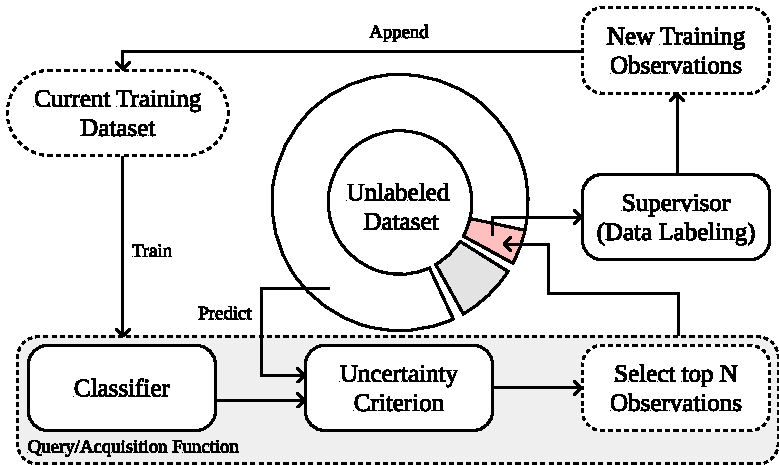
\includegraphics[width=.6\linewidth]{../analysis/al_iteration}
    \caption{%
        Diagram depicting a typical AL iteration. In the first iteration, the
        training set collected during the initialization process becomes the
        ``Current Training Dataset''.
    }~\label{fig:al_iteration}
\end{figure}

Research focused on AL has typically been focused on the specification of
$f_{acq}$~\cite{hospedales2011finding} and domain-specific applications, such
as malware detection~\cite{li2022boosting} or Land Use/Land Cover
classification~\cite{li2020label}. Acquisition functions can be divided into
two different categories~\cite{su2021cost, Kumar2020}: 

\begin{enumerate}

    \item Informative-based. These strategies use the classifier's output to
        assess the importance of each observation towards the performance of
        the classifier~\cite{Fu2013}.

    \item Representative-based. These strategies estimate the optimal set of
        observations that will optimize the classifier's
        performance~\cite{Kumar2020}.

\end{enumerate}

Although there are significant contributions toward the development of more
robust query functions and classifiers in AL, modifications to AL's basic
structure are rarely explored. In~\cite{Yoo2019} the authors introduce a loss
prediction module in the AL framework to replace the uncertainty criterion.
This model implements a second classifier to predict the expected loss of the
unlabeled observations (using the actual losses collected during the training
of the original classifier) and return the unlabeled observations with the
highest expected loss. However, this contribution is specific to deep neural
networks and was only tested for image classification.

\subsection{Data Augmentation}~\label{sec:data_augmentation}

Data Augmentation methods expand the training dataset by introducing new and
informative observations \cite{Behpour2019}. The production of artificial data
may be done via the introduction of perturbations on the
input~\cite{fonseca2021improving}, feature~\cite{DeVries2017}, or output
space~\cite{Behpour2019}. Data Augmentation methods may be divided into two
categories~\cite{Shorten2019}:

\begin{enumerate}
    \item Heuristic approaches attempt to generate new and relevant
        observations by applying a predefined procedure, usually incorporating
        some degree of randomness~\cite{Kashefi2020}. Since these methods
        typically occur in the input space, they require fewer data and
        computational power when compared to Neural Network methods. 
    \item Neural Network approaches, on the other hand, map the original input
        space into a lower-dimensional representation, known as the feature
        space~\cite{DeVries2017}. The generation of artificial data occurs in
        the feature space and is reconstructed into the input space. Although
        these methods allow the generation of less noisy data in
        high-dimensional contexts and more plausible artificial data, they are
        significantly more computationally intensive. 
\end{enumerate}

While some techniques may depend on the domain, others are domain-agnostic.
For example, Random Erasing~\cite{Zhong2020}, Translation, Cropping and
Flipping are examples of image data-specific augmentation methods. Other
methods, such as autoencoders, may be considered domain agnostic.

\subsection{Data Augmentation in Active Learning
}~\label{sec:data_augmentation_in_al}

The standard AL model can be complemented with a data augmentation function,
$f_{aug}(x_i;\tau)$, where $\tau$ defines the augmentation policy. In this
context, $\tau$ refers to the transformation applied and its hyperparameters
and $f_{aug}(x;\tau): \mathcal{D} \rightarrow \mathcal{D}_{aug}(\mathcal{D})$
produces a modified observation, $\tilde{x} \in
\mathcal{D}_{aug}(\mathcal{D})$ where $\mathcal{D}_{aug}(\mathcal{D})$ is the
set of modified observations. This involves the usage of a new set of data,
$\mathcal{D}_{train}^t = \mathcal{D}_{lab}^t \cup \mathcal{D}_{aug}^t$, to
train the classifier.


As found in Section~\ref{sec:active_learning_methods}, improvements proposed
in the AL framework are primarily focused on modifications of the classifier
or query strategy. Furthermore, the few recent AL contributions implementing
data augmentation were all (except one) applied to the computer vision or
natural language processing (NLP) realm. 

% Pipelined approach
The only AL model found that uses data augmentation outside of the computer
vision or NLP domains implements a pipelined approach, described
in~\cite{Fonseca2021}. In this study, the AL model proposed is applied for
tabular data using an oversampling data augmentation policy (\textit{i.e.},
the artificial data was only generated to balance the target class
frequencies). However, this AL model was applied in a Land Use/Land Cover
classification context with specific characteristics that are not necessarily
found in other supervised learning problems. Specifically, these types of
datasets are high dimensional and have limited data variability within each
class (\textit{i.e.,} cohesive spectral signatures within classes) due to
their geographical proximity. Furthermore, this method does not allow
augmentation policy optimization (i.e., every hyperparameter has to be
hardcoded \textit{a priori}).

The Bayesian Generative Active Deep Learning (BGDAL)~\cite{tran2019bayesian}
is another example of a pipelined combination of $f_{acq}$ and $f_{aug}$,
applied to image classification. BGDAL uses a Variational AutoEncoder (VAE)
architecture to generate artificial observations. However, the proposed model
is computationally expensive, requires a large data pool to train the VAE, and
is not only dependent on the quality of the augmentations performed, but also
on the performance of the discriminator and classifiers used.

% Look ahead data augmentation
The method proposed in~\cite{Kim2021}, Look-Ahead Data Acquisition for Deep
Active Learning, implements data augmentation to train a deep-learning
classifier. However, adapting existing AL applications to use this approach is
often impractical and implies the usage of image data since the augmentations
used are image data specific and occur on the unlabeled observations, before
the unlabeled data selection.

% VAE adversarial Active Learning (2019)
The Variational Adversarial Active Learning (VAAL)
model~\cite{sinha2019variational} is a deep AL approach to image
classification that uses as inputs the embeddings produced by a VAE into a
secondary classifier, working as $f_{acq}$, to predict if $x_i \in
\mathcal{D}$ belongs to $\mathcal{D}_{pool}$. The $n$ true positives with the
highest certainty are labeled by the supervisor and $\mathcal{D}_{pool}$ and
$\mathcal{D}_{lab}$ are updated as described in
Section~\ref{sec:active_learning_methods}. The Task-aware VAAL
model~\cite{kim2021task} extends the VAAL model by introducing a ranker, which
consists of the Learning Loss module introduced in~\cite{Yoo2019}. These
models use data augmentation techniques to train the different neural
network-based components of the proposed models. However, the AL components
used are specific image classification, computationally expensive and the
analysis of the effect of data augmentation in these AL models is not
discussed.

% Other applications
In~\cite{Ma2020}, the proposed AL method was explicitly designed for image
data classification, where a deep learning model was implemented as a
classifier, but its architecture is not described, the augmentation policies
used are unknown and the results reported correspond to single runs of the
discussed model. The remaining AL models found implement data augmentation for
NLP applications, in~\cite{Quteineh2020, Li2021framework}. However, these
methods were designed for specific applications within that domain and are not
necessarily transferable to other domains or tasks.

\section{Proposed Method}~\label{sec:proposed_method}

Based on the literature found on AL, most of the contributions and novel
implementations of AL algorithms have focused on the improvement of the
choice/architecture of the classifier or the improvement of the uncertainty
criterion. In addition, the resulting classification performance of AL-trained
classifiers is frequently inconsistent and marginally improve the
classification performance when compared to classifiers trained over the
entire training set. In addition, there is also significant variability in the
data selection efficiency during different runs of the AL iterative
process~\cite{Fonseca2021}.
 
This paper provides a context-agnostic AL framework for the integration of
Data Augmentation within AL, with the following contributions:

\begin{enumerate}
    \item Improvement of the AL framework by introducing a parameter tuning
        stage only using the labeled dataset available at the current
        iteration (\textit{i.e.,} no labeled hold-out set is needed).
    \item Generalization of the generator module proposed in
        \cite{Fonseca2021} from oversampling techniques to any other data
        augmentation mechanism and/or policy.
    \item Implementation of data augmentation outside the Deep AL realm, which
        was not previously found in the literature.
    \item Analysis of the impact of Data Augmentation and Oversampling in AL
        over 15 different datasets of different domains, while comparing them
        with the standard AL framework.
\end{enumerate}

The proposed AL framework is depicted in Figure~\ref{fig:al_proposed}. The
generator element becomes an additional source of data and is expected to
introduce additional data variability into the training dataset. This aspect
should allow the classifier to generalize better and perform more consistently
over unseen observations. However, in this scenario, the amount of data to
generate per class at each iteration is unknown. Consequently, the
hyperparameter tuning step was introduced to estimate the optimal data
augmentation policy at each iteration. In our implementation, this step uses
the current training dataset to perform an exhaustive search over specified
generator parameters, tested over a 5-fold cross-validation method. The best
augmentation policy found is used to train the iteration's classifier in the
following step. This procedure is described in
Algorithm~\ref{alg:al-framework}.


\begin{figure}
	\centering
	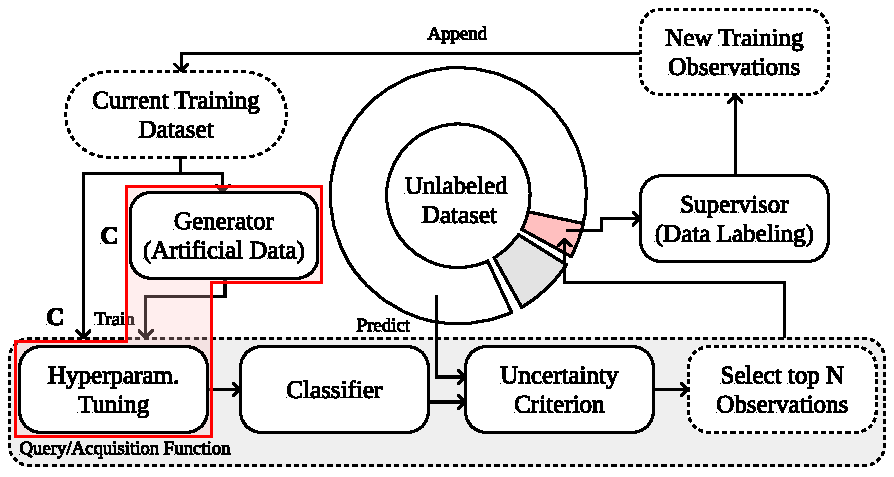
\includegraphics[width=.6\linewidth]{../analysis/al_proposed}
    \caption{%
        Diagram depicting the proposed AL iteration. The proposed
        modifications are marked with a boldface ``C.''
    }~\label{fig:al_proposed}
\end{figure}

We implemented a simple modification in the selection mechanism of the G-SMOTE
algorithm to show the effectiveness of data augmentation in an AL
implementation. We use the uncertainties produced by $f_{acq}$ to compute the
probabilities of observations to be selected for augmentation as an additional
parameter. This modification is described in Algorithm~\ref{alg:g-smote} 

\begin{algorithm}
    \SetKwInput{KwGiven}{Given}
    \SetKwProg{Fn}{Function}{:}{end}
    \caption{Proposed AL Framework (Single iteration)}\label{alg:al-framework}
    \DontPrintSemicolon%
    \KwGiven{$t \ge 1$, performance metric $f_{pm}$}
    \KwIn{$\mathcal{D}_{pool}$, $\mathcal{D}_{lab}$, $f_c$, $f_{aug}$,
    $f_{acq}$, $\tau_{grid}$, $k$, $n$}
    \KwOut{$\mathcal{D}_{pool}$, $\mathcal{D}_{lab}$}

    \Fn{ParameterTuning($f_c$, $f_{aug}$, $\tau_{grid}$, $\mathcal{D}_{lab}$,
    $k$)}{
        $p \leftarrow 0$ \\
        $\tau \leftarrow \emptyset$ \\
        $\{\mathcal{D}_{lab}^1, \ldots \mathcal{D}_{lab}^k\} \leftarrow
        \mathcal{D}_{lab}$
        \tcp*[f]{$\mathcal{D}_{lab}^n \cap \mathcal{D}_{lab}^m = \emptyset,
        \forall (n, m) \in {1, \ldots, k}$} \\
        \ForAll{$\tau' \in \tau_{grid}$}{
            $p' \leftarrow \emptyset$ \\
            \ForAll{
                $\mathcal{D}_{lab}^i \in \{\mathcal{D}_{lab}^1, \ldots
                \mathcal{D}_{lab}^k\}$
            }{
                $\mathcal{D}_{test}' \leftarrow \mathcal{D}_{lab}^i$ \\
                $\mathcal{D}_{train}' \leftarrow \mathcal{D}_{lab} \setminus
                \mathcal{D}_{lab}^i$ \\
                $\mathcal{D}_{train}' \leftarrow f_{aug}(\mathcal{D}_{train}';
                \tau')$ \\
                \textbf{train} $f_c$ using $\mathcal{D}_{train}'$ \\
                $p' \leftarrow p' \cup \{f_{pm}(f_c(\mathcal{D}_{test}))\}$
            }
            $p' \leftarrow \frac{\sum_{x_i \in p'}{x_i}}{k}$ \\
            \If{$p' > p$}{
                $p \leftarrow p'$ \\
                $\tau \leftarrow \tau'$
            }
        }
        \Return $\tau$
    }

    \Begin{
        $\tau \leftarrow ParameterTuning(f_c, f_{aug}, \tau_{grid},
        \mathcal{D}_{lab}, k)$ \\
        $\mathcal{D}_{train} \leftarrow f_{aug}(\mathcal{D}_{lab}; \tau)$ \\
        \textbf{train} $f_c$ using $\mathcal{D}_{train}$ \\
        $\mathcal{D}_{new} = \arg\max_{\mathcal{D}_{pool}'\subset
        \mathcal{D}_{pool}, |\mathcal{D}_{pool}'|=n} \sum_{x \in
        \mathcal{D}_{pool}'}{f_{acq}(x; f_c)}$ \\
        \textbf{annotate} $\mathcal{D}_{new}$ \\
        $\mathcal{D}_{pool} \leftarrow \mathcal{D}_{pool} \setminus
        \mathcal{D}_{new}$ \\
        $\mathcal{D}_{lab} \leftarrow \mathcal{D}_{lab} \cup
        \mathcal{D}_{new}$ \\
    }

\end{algorithm}

This modification facilitates the usage of G-SMOTE beyond its original
oversampling purposes. However, in this paper, the data augmentation
strategies are also used to ensure that class frequencies are balanced.
Furthermore, the amount of artificial data produced for each class is defined
by the \textit{augmentation factor}, $\alpha_{af}$, which represents a
percentage of the majority class $C_{maj}$ (\textit{e.g.,} an augmentation
factor of $1.2$ will ensure there are $count(C_{maj}) \times 1.2$ observations
in every class). In this paper's experiment, the data generation mechanism is
similar to the one in~\cite{Fonseca2021}. This factor allows the direct
comparison of the two frameworks and establishes a causality of the
performance variations to the data generation mechanism (\textit{i.e.,}
augmentation vs normal oversampling) and hyperparameter tuning steps.
However, in this case, the hyperparameter tuning is solely going to be used
for augmentation policy optimization. 

\begin{algorithm}[t]
    \SetKwInput{KwGiven}{Given}
    \SetKwProg{Fn}{Function}{:}{end}
    \caption{G-SMOTE Modified for Data Augmentation in AL}\label{alg:g-smote}
    \DontPrintSemicolon% 
    \KwGiven{$t \ge 1$, $\mathcal{D}_{lab}^t \ne \emptyset$,
    $\mathcal{D}_{lab} = \mathcal{D}_{lab}^{min} \cup \mathcal{D}_{lab}^{maj}$, \textit{GSMOTE}}
    \KwIn{$\mathcal{D}_{pool}^t$, $\mathcal{D}_{lab}^t$, $f_c^{t-1}$,
    $f_{acq}$, $\tau$}
    \KwOut{$\mathcal{D}_{train}^t$}

    \Fn{DataSelection($\mathcal{D}_{lab}^t$, $f_{acq}$, $f_c^{t-1}$)}{%
        $U \leftarrow \emptyset$ \\ 
        $P \leftarrow \emptyset$ \\ 
        $p_s \sim \mathcal{U}(0, 1)$ \\
        \ForAll{$x_i \in \mathcal{D}_{lab}^t$}{
            $u_{x_i} \leftarrow f_{acq}(x_i; f_c^{t-1})$\\
            $U \leftarrow U \cup \{u_{x_i}\}$
        }
        \ForAll{$u_{x_i} \in U$}{
            $p_{x_i} \leftarrow \frac{u_{x_i}}{\sum{U}} + \sum{P}$ \\
            $P \leftarrow P \cup \{p_{x_i}\}$
        }
        $i \leftarrow argmax(P < p_s)$ \\
        \Return i-th element in $\mathcal{D}_{lab}^t$
    }
    \Begin{
        $\mathcal{D}_{aug}^{min} \leftarrow \emptyset$ \\
        $\mathcal{D}_{aug}^{maj} \leftarrow \emptyset$ \\
        $\alpha_{af}, \alpha_{trunc}, \alpha_{def} \leftarrow \tau$ \\
        $N \leftarrow count(C_{maj}) \times \alpha_{af}$ \\
        
        \ForAll{
            $\mathcal{D}'_{aug} \in \{\mathcal{D}_{aug}^{min},
            \mathcal{D}_{aug}^{maj}\}$, $\mathcal{D}'_{lab} \in \{\mathcal{D}_{lab}^{min},
            \mathcal{D}_{lab}^{maj}\}$
        }{
            \While{
                $|\mathcal{D}'_{aug}| < N$
            }{
                $x_{center} \leftarrow DataSelection(\mathcal{D}'_{lab},
                f_{acq}, f_c^{t-1})$ \\
                $x_{gen} \leftarrow GSMOTE(x_{center}, \mathcal{D}_{lab}^t, \alpha_{trunc},
                \alpha_{def})$ \\
                $\mathcal{D}'_{aug} \leftarrow \mathcal{D}'_{aug} \cup
                \{x_{gen}\}$
            }
        }
        $\mathcal{D}_{aug} \leftarrow \mathcal{D}_{aug}^{min} \cup \mathcal{D}_{aug}^{maj}$ \\
        $\mathcal{D}_{train}^t \leftarrow \mathcal{D}_{lab}^t \cup
        \mathcal{D}_{aug}$
    }
\end{algorithm}

In the proposed framework, we (1) generalize the generator module to accept
any data augmentation method or policy and (2) a hyperparameter tuning module
to estimate the optimal data augmentation policy. This framework was designed
to be task-agnostic. Specifically, any data augmentation method
(domain-specific or not) may be applied, as well as any other parameter search
method. It is also expected to be compatible with other AL modifications,
including those that do not affect solely the classifier or uncertainty
criterion, such as the one proposed in~\cite{Yoo2019}.
 
\section{Methodology}~\label{sec:methodology}

This section describes the different elements included in the experimental
procedure. The datasets used were acquired in open data repositories. Their
sources and preprocessing steps are defined in Subsection~\ref{sec:datasets}.
The classifiers used in the experiment are defined in
Subsection~\ref{sec:machine_learning_algorithms}. The metrics chosen to
measure AL performance and overall classification performance are defined in
Subsection~\ref{sec:evaluation_metrics}. The experimental procedure is
described in Subsection~\ref{sec:experimental_procedure}. The implementation
of the experiment and resources used to do so are described in
Subsection~\ref{sec:software_implementation}.

The methodology developed serves a two-fold purpose: (1) Compare
classification performance once all the AL procedures are completed
(\textit{i.e.,} optimal performance of a classifier trained via iterative data
selection) and (2) Compare the amount of data required to reach specific
performance thresholds (\textit{i.e.,} the number of AL iterations required to
reach similar classification performances).
 
\subsection{Datasets}~\label{sec:datasets}

The datasets used to test the proposed method are publicly available in open
data repositories. Specifically, they were retrieved from
\href{https://www.openml.org/}{OpenML} and the
\href{https://archive.ics.uci.edu/}{UCI Machine Learning Repository}. They
were chosen considering diverse application domains, imbalance ratios,
dimensionality and number of target classes, all of them focused on
classification tasks. The goal is to demonstrate the performance of the
different AL frameworks in various scenarios and domains. The data
preprocessing approach was similar across all datasets.
Table~\ref{tab:datasets_description} describes the key properties of the
15 preprocessed datasets where the experimental procedure was applied. 
 
\begin{table}[H]
    \centering
    \setlength{\tabcolsep}{2pt}
    \caption{\label{tab:datasets_description}
        Description of the datasets collected after data preprocessing. The
        sampling strategy is similar across datasets. Legend: (IR) Imbalance
        Ratio
    }
    \pgfplotstabletypeset[
        col sep=comma,
        string type,
        every head row/.style={%
            before row=\toprule,
            after row=\midrule
        },
        every last row/.style={after row=\bottomrule},
    ]{../analysis/datasets_description.csv}
\end{table}

The data preprocessing pipeline is depicted as a flowchart in
Figure~\ref{fig:data_preprocessing}. The missing values are removed from each
dataset by removing the corresponding observations. This step ensures that the
input data in the experiment is kept as close to its original form as
possible. The non-metric features (\textit{i.e.,} binary, categorical, and
ordinal variables) were removed since the application of G-SMOTE is limited to
continuous and discrete features. The datasets containing over 2000
observations were downsampled in order to maintain the datasets to a
manageable size. The data sampling procedure preserves the relative class
frequency of the dataset, in order to maintain the Imbalance Ratio (IR)
originally found in each dataset (where $IR =
\frac{count(C_{maj})}{count(C_{\min})}$). The remaining features of each
dataset are scaled to the range of $[-1, 1]$ to ensure a common range across
features.

\begin{figure}[t]
	\centering
	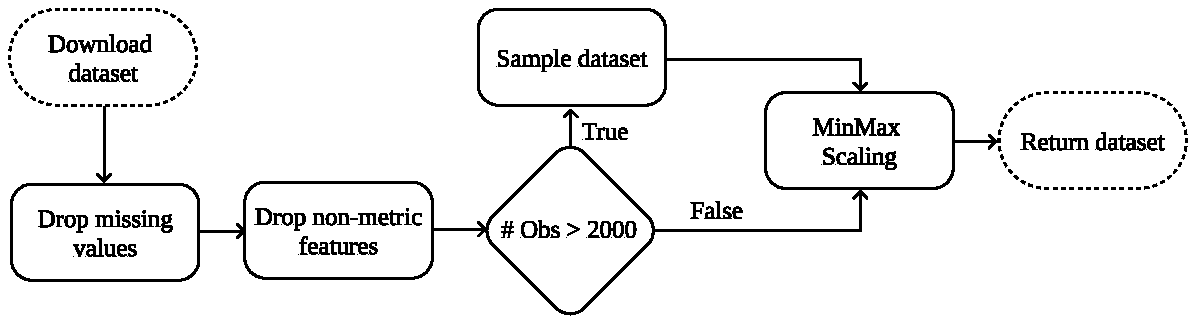
\includegraphics[width=.8\linewidth]{../analysis/data_preprocessing}
    \caption{%
        Data preprocessing pipeline.
    }~\label{fig:data_preprocessing}
\end{figure}

The preprocessed datasets were stored into an SQLite database file and is
available along with the experiment's source code in the project's GitHub
repository (see Subsection~\ref{sec:software_implementation}).
 
\subsection{Machine Learning Algorithms}~\label{sec:machine_learning_algorithms}

We used a total of four classification algorithms and a heuristic data
augmentation mechanism. The choice of classifiers was based on the popularity
and family of the classifiers (tree-based, nearest neighbors-based,
ensemble-based and linear models). Our proposed method was tested using a
Decision Tree (DT)~\cite{Wu1975}, a K-nearest neighbors classifier
(KNN)~\cite{Cover1967}, a Random Forest Classifier (RF)~\cite{Ho1995} and a
Logistic Regression (LR)~\cite{Nelder1972}. Since the target variables are
multi-class, the LR classifier was implemented using the one-versus-all
approach. The predicted class is assigned to the label with the highest
likelihood.
 
The oversampler G-SMOTE was used as a data augmentation method. The typical
data generation policy of oversampling methods is to generate artificial
observations on non-majority classes such that the number of majority class
observations matches those of each non-majority class. We modified this data
generation policy to generate observations for all classes, as a percentage of
the number of observations in the majority class. In addition, the original
G-SMOTE algorithm was modified to accept data selection probabilities based on
classification uncertainty. These modifications are discussed in
Section~\ref{sec:proposed_method}.

Every AL procedure was tested with different selection criteria: Random
Selection, Entropy, and Breaking Ties. The baseline used is the standard AL
procedure. As a benchmark, we add the AL procedure using G-SMOTE as a standard
oversampling method, as proposed in~\cite{Fonseca2021}. Our proposed method
was implemented using G-SMOTE as a data augmentation method to generate
artificial observations for all classes, while still balancing the class
distribution, as described in Section~\ref{sec:proposed_method}. 
 
\subsection{Evaluation Metrics}~\label{sec:evaluation_metrics}

Considering the imbalanced nature of the datasets used in the experiment,
commonly used performance metrics such as Overall Accuracy (OA), although
being intuitive to interpret, are insufficient to quantify a model's
classification performance~\cite{Jeni2013}. The Cohen's Kappa performance
metric, similar to OA, is also biased towards high-frequency classes since its
definition is closely related to the OA metric, making its behavior consistent
with OA~\cite{Fatourechi2008}. However, these metrics remain popular choices
for the evaluation of classification performance. Other performance metrics
like $Precision = \frac{TP}{TP+TN}$, $Recall = \frac{TP}{TP+FN}$ or
$Specificity = \frac{TN}{TN + FP}$ are calculated as a function of True/False
Positives (TP and FP) and True/False Negatives (TN and FN) and can be used on
a per-class basis instead. In a multiple dataset scenario with varying amounts
of target classes and meanings, comparing the performance of different models
using these metrics becomes impractical.
 
Based on the recommendations found in~\cite{Jeni2013, Kubat1997}, we used two
metrics found to be less sensitive to the class imbalance bias, along with OA
as a reference for easier interpretability:

\begin{itemize}
    \item The Geometric-mean scorer (G-mean) consists of the geometric mean of
        Specificity and Recall~\cite{Kubat1997}. Both metrics are calculated
        in a multi-class context considering a one-versus-all approach. For
        multi-class problems, the G-mean scorer is calculated as its average
        per class values: 
        
        \begin{equation*}
            \textit{G-mean} = \sqrt{\overline{Sensitivity} \times
            \overline{Specificity}}
        \end{equation*}

    \item The F-score metric consists of the harmonic mean of Precision and
        Recall. The two metrics are also calculated considering a
        one-versus-all approach. The F-score for the multi-class case can be
        calculated using its average per class values~\cite{Jeni2013}:

        \begin{equation*}
            \textit{F-score}=2\times\frac{\overline{Precision} \times
            \overline{Recall}}{\overline{Precision} + \overline{Recall}}
        \end{equation*}

    \item The OA consists of the number of TP divided by the total amount of
        observations. Considering $c$ as the label for the different classes
        present in a target class, OA is given by the following formula:

        \begin{equation*}
            \textit{OA} = \frac{\sum\limits_{c}{\text{TP}_{c}}}{%
		    	      \sum\limits_{c}{(\text{TP}_{c}+\text{FP}_{c})}}
        \end{equation*}
\end{itemize}

The comparison of the performance of AL frameworks is based on its data
selection and augmentation efficacy. Specifically, an efficient data
selection/generation policy allows the production of classifiers with high
performance on unseen data while using as least non-artificial training data
as possible. We follow the recommendations found in~\cite{Kottke2017}. To
measure the performance of the different AL setups, the performance of an AL
setup will be compared using two AL-specific performance metrics:

\begin{itemize}

    \item Area Under the Learning Curve (AULC). It is the sum of the
        classification performance over a validation/test set of the
        classifiers trained of all AL iterations. The resulting AULC scores
        are fixed within the range $[0, 1]$ by dividing the AULC scores by the
        total amount of iterations (\textit{i.e.}, the maximum performance
        area) to facilitate the interpretability of this metric.

    \item Data Utilization Rate (DUR)~\cite{Reitmaier2013}. Measures the
        percentage of training data required to reach a given performance
        threshold, as a ratio of the percentage of training data required by
        the baseline framework. This metric is also presented as a percentage
        of the total amount of training data, without making it relative to
        the baseline framework. The DUR metric is measured at 45 different
        performance thresholds, ranging between $[0.10, 1.00]$ at a 0.02 step.

\end{itemize}
 
\subsection{Experimental Procedure}~\label{sec:experimental_procedure}

The evaluation of different active learners in a live setting is generally
expensive, time-consuming, and prone to human error. Instead, a common
practice is to compare them in an offline environment using labeled
datasets~\cite{Kagy2019}. Since the dataset is already labeled, the annotation
process is done at zero cost in this scenario.
Figure~\ref{fig:experimental_procedure} depicts the experiment designed for
one dataset over a single run. 
 
A single run starts with the splitting of a preprocessed dataset into five
different partitions, stratified according to the class frequencies of the
target variable using the K-fold Cross Validation method. During this run, an
active learner or classifier is trained five times using a different partition
as the Test set each time. For each training process, a validation set
containing 25\% of the subset is created and is used to measure the data
selection efficiency (\textit{i.e.,} AULC and DUR using the classification
performance metrics, specific to AL). Therefore, for a single training
procedure, 20\% of the original dataset is used as the validation set, 20\% is
used as the Test set and 60\% is used as the training set. The AL simulations
and the classifiers' training occur within the training set. However, the
classifiers used to find the maximum performance classification scores are
trained over the full training set. The AL simulations are run over a maximum
of 50 iterations (including the initialization step), adding 1.6\% of the
training set each time (\textit{i.e.,} all AL simulations use less than 80\%
of the training set). Once the training phase is completed, the Test set
classification scores are calculated using the trained classifiers. For the
case of AL, the classifier with the optimal validation set score is used to
estimate the AL's optimal classification performance over unseen data.

The process shown in Figure~\ref{fig:experimental_procedure} is repeated over
three runs using different random seeds over the 15 different datasets
collected. The final scores of each AL configuration and classifier correspond
to the average of the three runs and 5-fold Cross-Validation estimations
(\textit{i.e.,} the mean score of 15 fits, across 15 datasets).

\begin{figure}
	\centering
	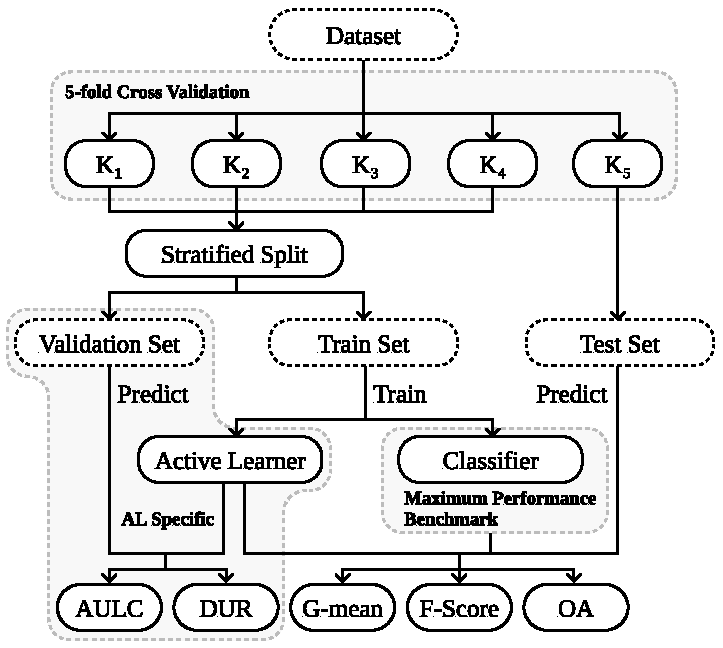
\includegraphics[width=.5\linewidth]{../analysis/experimental_procedure}
    \caption{%
        Experimental procedure flowchart. The preprocessed datasets are split
        into five folds. One of the folds is used to test the best-found
        classifiers using AL and the classifiers trained using the entire
        training dataset (containing the remaining folds). The training set is
        used to run both the AL simulations as well as train the normal
        classifiers. The validation set is used to measure AL-specific
        performance metrics over each iteration. We use different subsets for
        overall classification performance and AL-specific performance to
        avoid data leakage.
    }~\label{fig:experimental_procedure}
\end{figure}

The hyperparameters defined for the AL frameworks, Classifiers, and Generators
are shown in Table~\ref{tab:grid}. In the Generators table, we distinguish the
G-SMOTE algorithm working as a normal oversampling method from G-SMOTE-AUGM,
which generates additional artificial data on top of the usual oversampling
mechanism. Since the G-SMOTE-AUGM method is intended to be used with varying
parameter values (via within-iteration parameter tuning), the parameters were
defined as a list of various possible values.

\begin{table}
	\centering
    \caption{\label{tab:grid}
        Hyperparameter definition for the active learners, classifiers,
        and generators used in the experiment.
    }
	\begin{tabular}{lll}
		\toprule
		Active Learners & Hyperparameters                   & Inputs                         \\
		\midrule
		Standard        & \# initial obs.\                  & 1.6\%                          \\
                        & \# additional obs.\ per iteration & 1.6\%                          \\
                        & max.\ iterations + initialization & 50                             \\
                        & evaluation metrics                & G-mean, F-score, OA            \\
                        & selection strategy                & Random, Entropy, Breaking Ties \\
                        & within-iteration param.\ tuning   & None                           \\
                        & generator                         & None                           \\
                        & classifier                        & DT, LR, KNN, RF                \\
        Oversampling    & generator                         & G-SMOTE                        \\
        Proposed        & generator                         & G-SMOTE-AUGM                   \\
                        & within-iteration param.\ tuning   & Grid Search K-fold CV          \\
		\toprule
		Classifier      &                                  &                                \\
		\midrule
        DT              & min.\ samples split              & 2                              \\
                        & criterion                        & gini                           \\
		LR              & maximum iterations               & 100                            \\
                        & multi-class                      & One-vs-All                     \\
		                & solver                           & liblinear                      \\
                        & penalty                          & L2 (Ridge)                     \\
		KNN             & \# neighbors                     & 5                              \\
                        & weights                          & uniform                        \\
                        & metric                           & euclidean                      \\
		RF              & min.\ samples split              & 2                              \\
		                & \# estimators                    & 100                            \\
                        & criterion                        & gini                           \\
		\toprule
		Generator       &                                  &                                \\
		\midrule
		G-SMOTE         & \# neighbors                     & 4                              \\
                        & deformation factor               & 0.5                            \\
                        & truncation factor                & 0.5                            \\
		G-SMOTE-AUGM    & \# neighbors                     & 3, 4, 5                        \\
                        & deformation factor               & 0.5                            \\
                        & truncation factor                & 0.5                            \\
                        & augmentation factor              & $[1.1, 2.0]$ at 0.1 step       \\
		\bottomrule
	\end{tabular}
\end{table}
 
\subsection{Software Implementation}~\label{sec:software_implementation}

The experiment was implemented using the Python programming language, along
with the Python libraries
\href{https://scikit-learn.org/stable/}{Scikit-Learn}~\cite{Pedregosa2011},
\href{https://imbalanced-learn.org/en/stable/}{Imbalanced-Learn}~\cite{JMLR:v18:16-365},
\href{https://geometric-smote.readthedocs.io/en/latest/?badge=latest}{Geometric-SMOTE}~\cite{Douzas2019},
\href{https://research-learn.readthedocs.io/en/latest/?badge=latest}{Research-Learn}
and
\href{https://mlresearch.readthedocs.io/en/latest/?badge=latest}{ML-Research}
libraries. All functions, algorithms, experiments, and results are provided on
the \href{https://github.com/joaopfonseca/publications/}{project's GitHub
repository}.

\section{Results \& Discussion}~\label{sec:results_discussion}

In a multiple dataset experiment, the analysis of results should not rely upon
the average performance scores across datasets uniquely. The domain of
application and fluctuations of performance scores between datasets make the
analysis of these averaged results less accurate. Instead, it is generally
recommended to use the mean ranking scores to extend the
analysis~\cite{Demsar2006}. Since mean performance scores are still intuitive
to interpret; we will present and discuss both results. The rank values are
assigned based on the mean scores of three different 5-fold Cross-Validation
runs (15 performance estimations per dataset) for each combination of dataset,
AL configuration, classifier, and performance metric.
 
\subsection{Results}~\label{sec:results}

The average rankings of the AL methods' AULC estimations are shown in
Table~\ref{tab:aulc_ranks}. The proposed method almost always improves AL
performance and ensures higher data selection efficiency.
 
\begin{table}[t]
	\centering
    \caption{%
        Mean rankings of the AULC metric over the different datasets (15),
        folds (5), and runs (3) used in the experiment. The proposed method
        constantly improves the results of the original framework and, on
        average, almost always improves the results of the oversampling
        framework.
    }\label{tab:aulc_ranks}
    \pgfplotstabletypeset[
        col sep=comma,
        string type,
        every head row/.style={%
            before row=\toprule,
            after row=\midrule
        },
        every last row/.style={after row=\bottomrule},
    ]{../analysis/mean_std_aulc_ranks.csv}
\end{table}
 
Table~\ref{tab:aulc_scores} shows the average AULC scores, grouped by the
classifier, Evaluation Metric and AL framework. The performance of the
proposed method is almost always superior when considering the F-score and
G-mean. On some occasions, the average AULC score is significantly improved
when compared with the oversampling AL method.

\begin{table}[H]
	\centering
    \setlength{\tabcolsep}{2.5pt}
    \caption{\label{tab:aulc_scores}
        Average AULC of each AL configuration tested. Each AULC score is
        calculated using the performance scores of each iteration in the
        validation set. By the end of the iterative process, each AL
        configuration used a maximum of 80\% instances of the 60\% instances
        that compose the training sets (\textit{i.e.,} 48\% of the entire
        preprocessed dataset).
    }
    \pgfplotstabletypeset[
        col sep=comma,
        string type,
        every head row/.style={%
            before row=\toprule,
            after row=\midrule
        },
        every last row/.style={after row=\bottomrule},
    ]{../analysis/mean_std_aulc_scores.csv}
\end{table}

The average DUR scores were calculated for various G-mean thresholds, varying
between 0.1 and 1.0 at a 0.02 step (45 different thresholds in total).
Table~\ref{tab:optimal_data_utilization} shows the results obtained for these
scores starting from a G-mean score of 0.6 and was filtered to show the
thresholds ending with 0 or 6 only. In most cases, the proposed method reduces
the amount of data annotation required to reach each G-mean score threshold.

\begin{table}[H]
    \centering
    \setlength{\tabcolsep}{2.5pt}
    \caption{\label{tab:optimal_data_utilization}
        AL algorithms' mean data utilization as a percentage of the
        training set.
    }
    \pgfplotstabletypeset[
        col sep=comma,
        string type,
        every head row/.style={%
            before row=\toprule,
            after row=\midrule
        },
        every last row/.style={after row=\bottomrule},
    ]{../analysis/optimal_data_utilization.csv}
\end{table}

The DUR scores relative to the Standard AL method are shown in
Figure~\ref{fig:dur}. A DUR below 1 means that the Proposed/Oversampling
method requires less data than the Standard AL method to reach the same
performance threshold. For example, running an AL simulation using the KNN
classifier requires 80.7\% of the amount of data required by the Standard AL
method using the same classifier to reach an F-Score of 0.62 (\textit{i.e.,}
requires 19.3\% less data).

\begin{figure}[H]
	\centering
	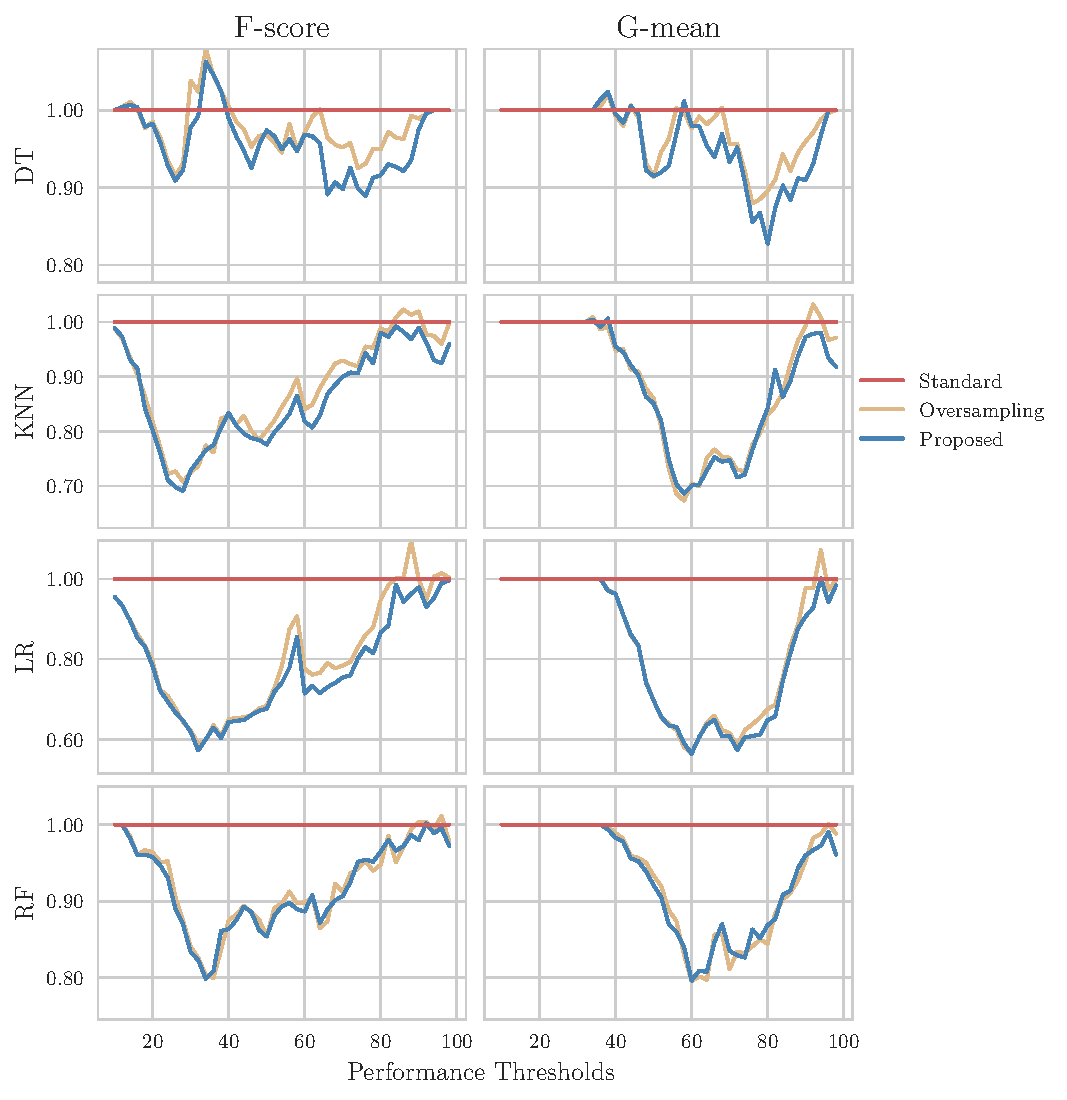
\includegraphics[width=.8\linewidth]{../analysis/data_utilization_rate}
    \caption{%
        Mean data utilization rates. The y-axis shows the percentage of data
        (relative to the baseline AL framework) required to reach the
        different performance thresholds.
    }~\label{fig:dur}
\end{figure}

The comparison of mean optimal classification scores of AL methods with
Classifiers (using the entire training set, without AL) is shown in
Table~\ref{tab:optimal_mean_std_scores}. Aside from the case of overall
accuracy, the proposed AL method produces classifiers that almost consistently
outperform classifiers using the whole training set (\textit{i.e.,} the ones
labeled as MP).

\begin{table}[H]
    \centering
    \caption{\label{tab:optimal_mean_std_scores}
        Optimal classification scores. The Maximum Performance (MP)
        classification scores are calculated using classifiers trained using
        the entire training set.
    }
    \pgfplotstabletypeset[
        col sep=comma,
        string type,
        every head row/.style={%
            before row=\toprule,
            after row=\midrule
        },
        every last row/.style={after row=\bottomrule},
    ]{../analysis/optimal_mean_std_scores.csv}
\end{table}

\subsection{Statistical Analysis}~\label{sec:statistical-analysis}

When checking for statistical significance in a multiple dataset context it is
critical to account for the multiple comparison problem. Consequently, our
statistical analysis focuses on the recommendations found
in~\cite{Demsar2006}. Overall, we perform three statistical tests. The
Friedman test~\cite{Friedman1937} is used to understand whether there is a
statistically significant difference in performance between the three AL
frameworks. As \textit{post hoc} analysis, the Wilcoxon signed-rank
test~\cite{Wilcoxon1945} was utilized to check for statistical significance
between the performance of the proposed AL method and the oversampling AL
method across datasets. As a second \textit{post hoc} analysis, the
Holm-Bonferroni~\cite{Holm1979} method was employed to check for statistical
significance between the methods using data generators and the Standard AL
framework across classifiers and evaluation metrics.
 
Table~\ref{tab:friedman_test} displays the \textit{p-values} obtained with the
Friedman test. The difference in performance across AL frameworks is
statistically significant at a level of $\alpha = 0.05$ regardless of the
classifier or evaluation metric being considered.

\begin{table}[t]
	\centering
    \caption{%
        Friedman test results. Statistical significance is tested at a level
        of $\alpha = 0.05$. The null hypothesis is that there is no difference
        in the classification outcome across oversamplers.
    }\label{tab:friedman_test}
    \pgfplotstabletypeset[
        col sep=comma,
        string type,
        every head row/.style={%
            before row=\toprule,
            after row=\midrule
        },
        every last row/.style={after row=\bottomrule},
    ]{../analysis/friedman_test.csv}
\end{table}

Table~\ref{tab:wilcoxon_test} contains the \textit{p-values} obtained with the
Wilcoxon signed-rank test. The proposed method was able to outperform both the
standard AL framework, as well as the AL framework using a typical
oversampling policy with statistical significance in 14 and 12 out of 15
datasets, respectively.

\begin{table}[H]
	\centering
    \caption{%
        Adjusted p-values using the Wilcoxon signed-rank method. Bold values
        are statistically significant at a level of $\alpha = 0.05$. The null
        hypothesis is that the performance of the proposed framework is
        similar to that of the oversampling or standard framework.
    }\label{tab:wilcoxon_test}
    \pgfplotstabletypeset[
        col sep=comma,
        string type,
        every head row/.style={%
            before row=\toprule,
            after row=\midrule
        },
        every last row/.style={after row=\bottomrule},
    ]{../analysis/wilcoxon_test.csv}
\end{table}

The \textit{p-values} shown in Table~\ref{tab:holms_test} refer to the results
of the Holm-Bonferroni test. The proposed method's superior performance was
statistically significant in 9 out of 12 cases. 

\begin{table}
	\centering
    \caption{%
        Adjusted p-values using the Holm-Bonferroni method. Bold values are
        statistically significant at a level of $\alpha = 0.05$. The null
        hypothesis is that the Oversampling or Proposed method does not
        perform better than the control method (Standard AL framework).
    }\label{tab:holms_test}
    \pgfplotstabletypeset[
        col sep=comma,
        string type,
        every head row/.style={%
            before row=\toprule,
            after row=\midrule
        },
        every last row/.style={after row=\bottomrule},
    ]{../analysis/holms_test.csv}
\end{table}

\subsection{Discussion}~\label{sec:sub_discussion}

In this paper, we study the application of data augmentation methods through
the modification of the standard AL framework. This is done to further reduce
the amount of labeled data required to produce a reliable classifier, at the
expense of artificial data generation.
 
% a different data generation strategy
% - Superiority of AL proposed vs standard (AULC + statistical analysis)
In Table~\ref{tab:aulc_ranks}, we found that the proposed method was able to
outperform the Standard AL framework in all scenarios. Except for the overall
accuracy metric, the mean rankings are consistent with the mean AULC scores
found in Table~\ref{tab:aulc_scores}, while showing performance improvements
between the proposed method and both the standard and oversampling methods.
The Friedman test in Table~\ref{tab:friedman_test} showed that the difference
in the performance of these AL frameworks are statistically significant,
regardless of the classifier or performance metric being used.
 
% parameter optimization within the iterative process of an AL procedure
% - Discuss consistency of results as compared with other methods (DUR metric)
The proposed method evidenced more consistent data utilization requirements in
most of the assessed G-mean score thresholds when compared to the remaining AL
methods, as seen in Table~\ref{tab:optimal_data_utilization}. For example, to
reach a G-mean score of 0.9 using the KNN and LR classifiers, the average
amount of data required with the Oversampling AL approach increased when
compared to the standard approach. However, the proposed method was able to
decrease the amount of data required in both situations. The robustness of the
proposed method is clearer in Figure~\ref{fig:dur}. In most cases, this method
was able to outperform the Oversampling method. At the same time, the proposed
method also addresses inconsistencies in situations where the Oversampling
method was unable to outperform the standard method.

% Data augmentation vs oversampling
The statistical analyses found in Tables~\ref{tab:wilcoxon_test}
and~\ref{tab:holms_test} revealed that the proposed method's superiority was
statistically significant in all datasets except three (Baseball, Usps, and
Volkert) and established statistical significance when compared to the
standard AL method for all combinations of classifier and performance metric,
except for three cases regarding the use of the overall accuracy metric. These
results show that the proposed method increased the reliability of the new AL
framework and improved the quality of the final classifier while using fewer
data.

% Usage of AL as a method to produce better performing classifiers, even in
% settings with fully labeled data
Even though it was not the core purpose of this study, we found that the
proposed AL method consistently outperformed the maximum performance
threshold. Specifically, in Table~\ref{tab:optimal_mean_std_scores}, the
performance of the classifiers originating from the proposed method was able
to outperform classifiers trained using the full training dataset in 9 out of
12 scenarios. This outcome suggests that the selection of a meaningful
training subset training dataset paired with data augmentation not only
matches the classification performance of ML algorithms, as it also improves
them. Even in a setting with fully labeled training data, the proposed method
may be used as a preprocessing technique to further optimize classification
performance.

% Future work and limitations
This study discussed the effect of data augmentation within the AL framework,
along with the exploration of optimal augmentation methods within AL
iterations. However, the conceptual nature of this study implies some
limitations. Specifically, the large number of experiments required to
test the method's efficacy, along with the limited computational power
available, led to a limited exploration of the grid search's potential. Future
work should focus on understanding how the usage of a more comprehensive
parameter tuning approach improves the quality of the AL method. In addition,
the proposed method was not able to outperform the standard AL method at
100\% of scenarios. The exploration of other, more complex data augmentation
techniques might further improve its performance by producing more
meaningful training observations. Specifically, in this study, we assume
that all datasets used follow a manifold, allowing the usage of G-SMOTE as a
data augmentation approach. However, this method cannot be used in more
complex, non-euclidean spaces. In this scenario, the usage of G-SMOTE is not
valid and might lead to the production of noisy data. Deep Learning-based data
augmentation techniques are able to address this limitation and improve the
overall quality of the artificial data being generated. We also
encountered significant standard errors throughout our experimental
results (see Subsection~\ref{sec:results}), consistent with the findings
in~\cite{Fonseca2021, Kottke2017}. This facet suggests that the usage of
more robust generators did not decrease the standard error of AL performance.
Instead, AL's performance variability is likely dependent on the quality of
its initialization.

\section{Conclusion}~\label{sec:conclusion}

The ability to train ML classifiers is usually limited to the availability of
labeled data. However, manually labeling data is often expensive, which makes
the usage of AL particularly appealing for selecting the most informative
observations and reducing the amount of required labeled data. On the other
hand, the introduction of data variability in the training dataset can also be
conducted via data augmentation. However, most, if not all, AL configurations
that use some form of data augmentation are domain and/or task-specific. These
methods typically apply deep learning approaches to both classification and
data augmentation. Consequently, they may not apply to other classification
tasks or when the available computational power is insufficient.

In this paper, we proposed a domain-agnostic AL framework that implements Data
Augmentation and hyperparameter tuning. We found that a heuristic Data
Augmentation algorithm is sufficient to improve the data selection efficiency
in AL\@. Specifically, the data augmentation method used almost always
increased AL performance, regardless of the target goal (\textit{i.e.,}
optimizing classification or data selection efficiency). The usage of data
augmentation reduced the number of iterations required to train a classifier
with a performance as good as (or better than) classifiers trained with the
entire training dataset (\textit{i.e.,} without using AL). In addition, the
proposed method reduced the size of the training dataset, which is expanded
with artificial data. 

With this revised AL configuration, data selection in AL iterations aims
towards observations that optimize the quality of the artificial data
produced. The substitution of less informative labeled data with artificial
data is especially useful in this context since it reduces some of the user
interaction necessary to reach a sufficiently informative dataset. In order
to further improve the proposed method, future work should (1) focus on the
development of methods with varying data augmentation policies depending on
the different input space regions, (2) develop augmentation-sensitive query
functions capable of avoiding the unnecessary selection of similar
observations from the unlabeled dataset and (3) understand the gap between
heuristic/input space data augmentation techniques and neural network/feature
space data augmentation techniques in an AL context better.

\section*{Acknowledgments}

This research was supported by three research grants of the Portuguese Foundation
for Science and Technology (``Fundação para a Ciência e a Tecnologia''),
references SFRH/BD/151473/2021, DSAIPA/DS/0116/2019 and PCIF/SSI/0102/2017.

\printbibliography%

\end{document}


